% Provenance (never printed): cycle 3 "La planete Terre" (natural phenomena
% and the risks they bring: storms, floods, droughts, earthquakes, eruptions;
% warnings and the right behaviour); see sources/book1/PROVENANCE.md.
% Book 1, grade 5, chapter 3.
\chapter{प्राकृतिक संकट}\label{ch:g5:natural-hazards}

शुक्रवार की शाम है। रेडियो पर संगीत रुकता है और एक शांत आवाज़ एक चेतावनी पढ़ती है:
आज रात \omterm{def:g1:landscapes-around-us:water}{तट} पर एक तेज़ \omterm{def:g5:natural-hazards:storm}{तूफ़ान} पहुँचेगा, बहुत तेज़ हवाओं और भारी \omterm{def:g4:clouds-rain-snow:precipitation}{बारिश} के साथ। लोगों
से कहा जाता है कि वे नौ बजे से घर के अंदर रहें, और जो कुछ भी हवा उड़ा ले जा सकती
है उसे बाँध दें या अंदर ले आएँ।

लीना का परिवार काम में लग जाता है। उसके पिता बग़ीचे की कुर्सियाँ और मेज़ कोठरी में
रख देते हैं। उसकी माँ जाँचती हैं कि टॉर्च चल रहे हैं, और अतिरिक्त बैटरियाँ रसोई की
मेज़ पर रख देती हैं। लीना पानी से दो बड़ी बोतलें भर लेती है। नौ बजे तक सब अंदर
हैं, और हवा अभी से
गरज रही है।

\begin{omfigure}
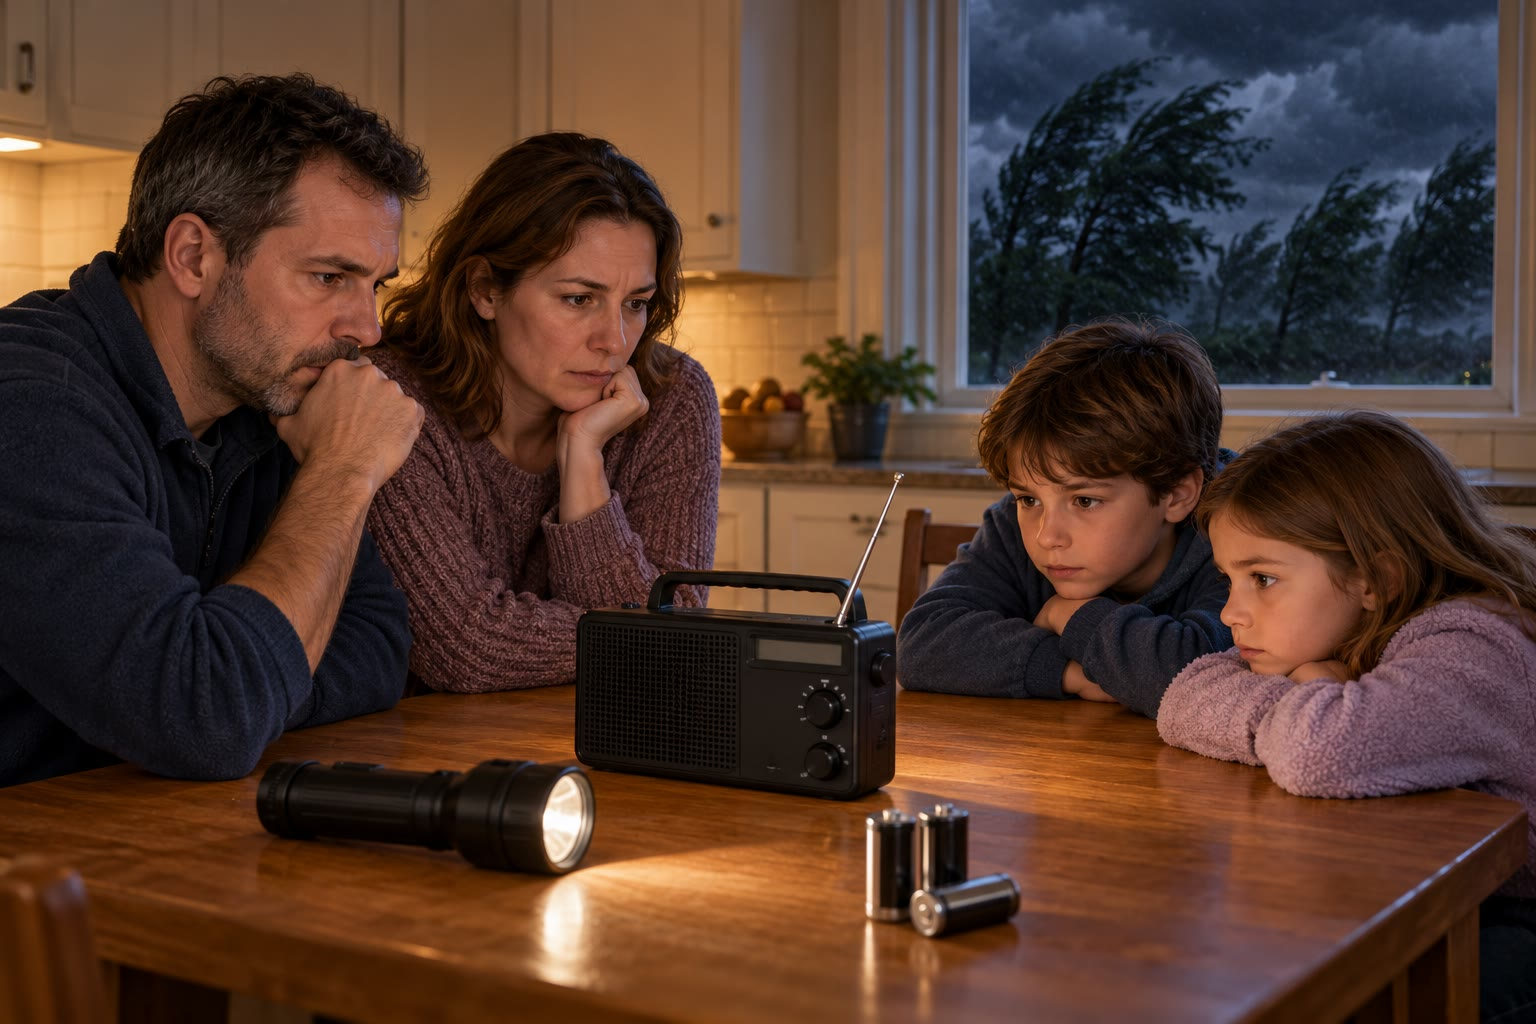
\includegraphics[width=0.5\linewidth]{images/book1/ai/g5-radio-warning.jpg}

{\small एक परिवार रेडियो पर \omterm{def:g5:natural-hazards:storm}{तूफ़ान} की चेतावनी सुनता है, टॉर्च और अतिरिक्त
बैटरियाँ तैयार रखकर।}
\end{omfigure}

\begin{recall}
\omterm{def:g4:volcanoes-earthquakes-first-look:volcano}{ज्वालामुखी} फूट सकता है, \omterm{def:g4:volcanoes-earthquakes-first-look:eruption}{लावा}, राख और गैस बाहर फेंकते हुए; \omterm{def:g4:volcanoes-earthquakes-first-look:earthquake}{भूकंप} ज़मीन का अचानक
काँपना है; \omterm{def:g4:volcanoes-earthquakes-first-look:earthquake}{भूकंप} में हम झुकते, ढकते और पकड़े रहते हैं
(\cref{ch:g4:volcanoes-earthquakes-first-look})। जिस \omterm{def:g1:landscapes-around-us:water}{नदी} को अपनी नाली की क्षमता से
ज़्यादा पानी मिलता है, वह अपने \omterm{def:g5:water-shapes-the-land:flood}{बाढ़} के \omterm{def:g1:landscapes-around-us:landform}{मैदान} पर \omterm{def:g5:water-shapes-the-land:flood}{बाढ़} ले आती है
(\cref{ch:g5:water-shapes-the-land})। हर जगह की अपनी \omterm{def:g5:weather-and-climate:climate}{जलवायु} है, और उष्ण,
शीतोष्ण और शीत कटिबंध \omterm{def:g3:continents-and-oceans:globe}{ग्लोब} के चारों ओर जाते हैं
(\cref{ch:g5:weather-and-climate})।
\end{recall}

\section{प्राकृतिक संकट क्या है}

प्रकृति हमेशा शांत नहीं रहती। हवा इतनी तेज़ चल सकती है कि पेड़ टूट जाएँ, \omterm{def:g1:landscapes-around-us:water}{नदियों} में
\omterm{def:g5:water-shapes-the-land:flood}{बाढ़} आ सकती है, ज़मीन काँप सकती है। ये घटनाएँ पृथ्वी के काम करने के ढंग का हिस्सा
हैं: वे लोगों के होने से बहुत पहले भी होती थीं, और आगे भी होती
रहेंगी।

\begin{definition}[प्राकृतिक संकट]\label{def:g5:natural-hazards:hazard}
\emph{प्राकृतिक संकट}\index{प्राकृतिक संकट} एक प्राकृतिक घटना है जो लोगों को
नुक़सान पहुँचा सकती है या उनकी बनाई चीज़ों को क्षति पहुँचा सकती है: \omterm{def:g5:natural-hazards:storm}{तूफ़ान}, \omterm{def:g5:water-shapes-the-land:flood}{बाढ़},
\omterm{def:g5:natural-hazards:drought}{सूखा}, \omterm{def:g4:volcanoes-earthquakes-first-look:earthquake}{भूकंप}, \omterm{def:g4:volcanoes-earthquakes-first-look:volcano}{ज्वालामुखी} \omterm{def:g4:volcanoes-earthquakes-first-look:eruption}{उद्गार}, \omterm{def:g5:natural-hazards:landslide}{भूस्खलन}{\ldots}
\end{definition}

\omterm{def:g5:natural-hazards:hazard}{प्राकृतिक संकटों} को हम इस आधार पर बाँट सकते हैं कि वे कहाँ से आते हैं: हवा से,
पानी से, या ज़मीन से।

\begin{omfigure}
\begin{tikzpicture}[font=\small, box/.style={draw, rounded corners=3pt,
    minimum width=4.2cm, minimum height=0.9cm, align=center}]
  \node[box, fill=cyan!15, font=\small\bfseries] (A) at (0,0) {हवा से};
  \node[box, fill=blue!15, font=\small\bfseries] (W) at (4.8,0) {पानी से};
  \node[box, fill=brown!25, font=\small\bfseries] (G) at (9.6,0) {ज़मीन से};
  \node[align=center, anchor=north] at (0,-0.7) {तूफ़ान\\उष्णकटिबंधीय चक्रवात\\लू\\सूखा};
  \node[align=center, anchor=north] at (4.8,-0.7) {बाढ़\\(नदियों से, भारी\\बारिश से, तूफ़ान में\\समुद्र से)};
  \node[align=center, anchor=north] at (9.6,-0.7) {भूकंप\\ज्वालामुखी उद्गार\\भूस्खलन};
  \node[draw, rounded corners=3pt, fill=gray!10, font=\small\bfseries,
    minimum width=5cm, minimum height=0.8cm] (N) at (4.8,1.5) {प्राकृतिक संकट};
  \draw[->] (N.south) -- (A.north);
  \draw[->] (N.south) -- (W.north);
  \draw[->] (N.south) -- (G.north);
\end{tikzpicture}

{\small \omterm{def:g5:natural-hazards:hazard}{प्राकृतिक संकट}, इस आधार पर बाँटे गए कि वे कहाँ से आते हैं।}
\end{omfigure}

\section{हवा से आने वाले संकट}

\begin{definition}[तूफ़ान]\label{def:g5:natural-hazards:storm}
\emph{तूफ़ान}\index{तूफ़ान} बहुत तेज़ हवा का समय है, आमतौर पर भारी \omterm{def:g4:clouds-rain-snow:precipitation}{बारिश} या \omterm{def:g4:clouds-rain-snow:precipitation}{हिम} के
साथ, और कभी-कभी गरज और बिजली के साथ।
\end{definition}

तेज़ \omterm{def:g5:natural-hazards:storm}{तूफ़ान} डालियाँ तोड़ता है, पेड़ गिराता है, छतों से खपरैल उखाड़ता है, और बग़ीचे की
कुर्सियों को खिड़कियों के पार फेंक सकता है। \omterm{def:g1:landscapes-around-us:water}{तट} पर उसकी हवा \omterm{def:g2:water-on-earth:ocean}{समुद्र} को किनारे की ओर
ढेर कर देती है और विशाल लहरों को समुद्री दीवारों के ऊपर से भेजती है।

पृथ्वी के सबसे शक्तिशाली \omterm{def:g5:natural-hazards:storm}{तूफ़ान} गरम उष्णकटिबंधीय \omterm{def:g2:water-on-earth:ocean}{समुद्रों} के ऊपर बनते हैं। वे विशाल,
घूमते हुए \omterm{def:g5:natural-hazards:storm}{तूफ़ान} हैं: अंतरिक्ष से वे \omterm{def:g4:clouds-rain-snow:cloud}{बादलों} के एक विशाल सर्पिल जैसे दिखते हैं, जिसके
बीच में एक शांत, साफ़ छेद होता है, उसकी आँख। आँख के चारों ओर सबसे तेज़ हवाएँ चलती
हैं। एक ही तरह के \omterm{def:g5:natural-hazards:storm}{तूफ़ान} के अलग-अलग \omterm{def:g2:water-on-earth:ocean}{महासागरों} में अलग-अलग नाम हैं: उत्तरी अटलांटिक
में और पूर्वी प्रशांत में उसे \emph{हरिकेन} कहते हैं, उत्तर-पश्चिमी प्रशांत में
\emph{टाइफ़ून}, और दक्षिणी प्रशांत और हिंद \omterm{def:g2:water-on-earth:ocean}{महासागर} में
\emph{उष्णकटिबंधीय चक्रवात}।
% ledger: noaa:cyclone-names

\begin{omfigure}
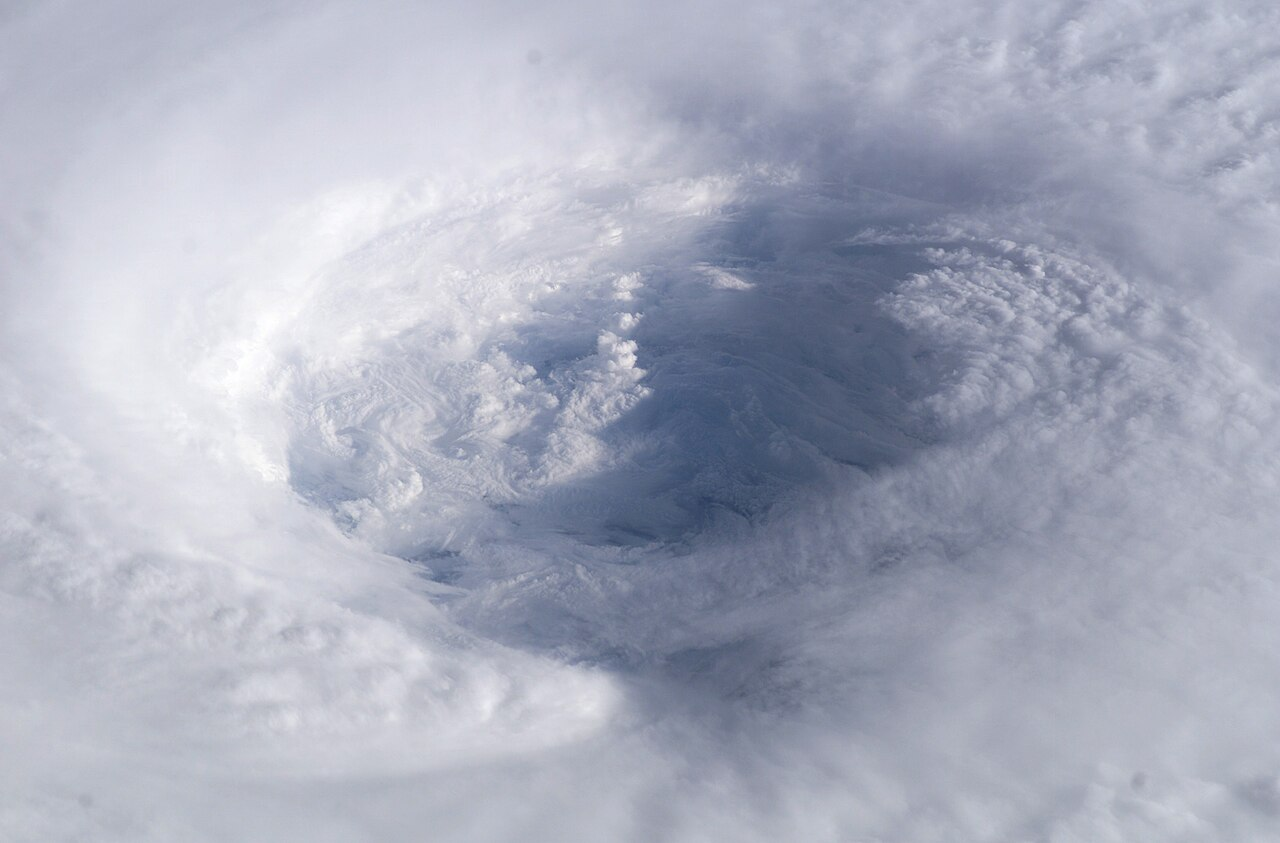
\includegraphics[width=0.5\linewidth]{images/book1/g5-hurricane-isabel-iss.jpg}

{\small सितंबर 2003 में अटलांटिक \omterm{def:g2:water-on-earth:ocean}{महासागर} के ऊपर हरिकेन इसाबेल की आँख में नीचे
झाँकते हुए, अंतरराष्ट्रीय अंतरिक्ष स्टेशन से: एक शांत केंद्र के चारों ओर \omterm{def:g4:clouds-rain-snow:cloud}{बादलों} की
एक दीवार। चित्र: नासा (सार्वजनिक डोमेन)।}
% ledger: nasa:isabel-iss
\end{omfigure}

हवा से आने वाले कुछ संकट धीमे और चुपचाप होते हैं। \emph{लू} कई दिनों और रातों का
ऐसा समय है जो सामान्य से बहुत ज़्यादा गरम होता है। वह सबसे बढ़कर बहुत बूढ़े लोगों,
शिशुओं और बीमारों के लिए ख़तरनाक है।

\begin{definition}[सूखा]\label{def:g5:natural-hazards:drought}
\emph{सूखा}\index{सूखा} महीनों या वर्षों तक का एक लंबा समय है, जिसमें उस जगह के
लिए सामान्य से बहुत कम \omterm{def:g4:clouds-rain-snow:precipitation}{बारिश} होती है। मिट्टी सूख जाती है, \omterm{def:g1:landscapes-around-us:water}{नदियाँ} और \omterm{def:g1:landscapes-around-us:water}{झीलें} सिकुड़
जाती हैं, फ़सलें मुरझाकर मर जाती हैं।
\end{definition}

\omterm{def:g5:natural-hazards:drought}{सूखा} धीरे-धीरे दबे पाँव आता है: कोई नहीं बता सकता कि वह किस दिन शुरू होता है। पर
लंबा \omterm{def:g5:natural-hazards:drought}{सूखा} किसानों को बिना फ़सल के और शहरों को पानी की कमी में छोड़ सकता है।

\begin{omfigure}
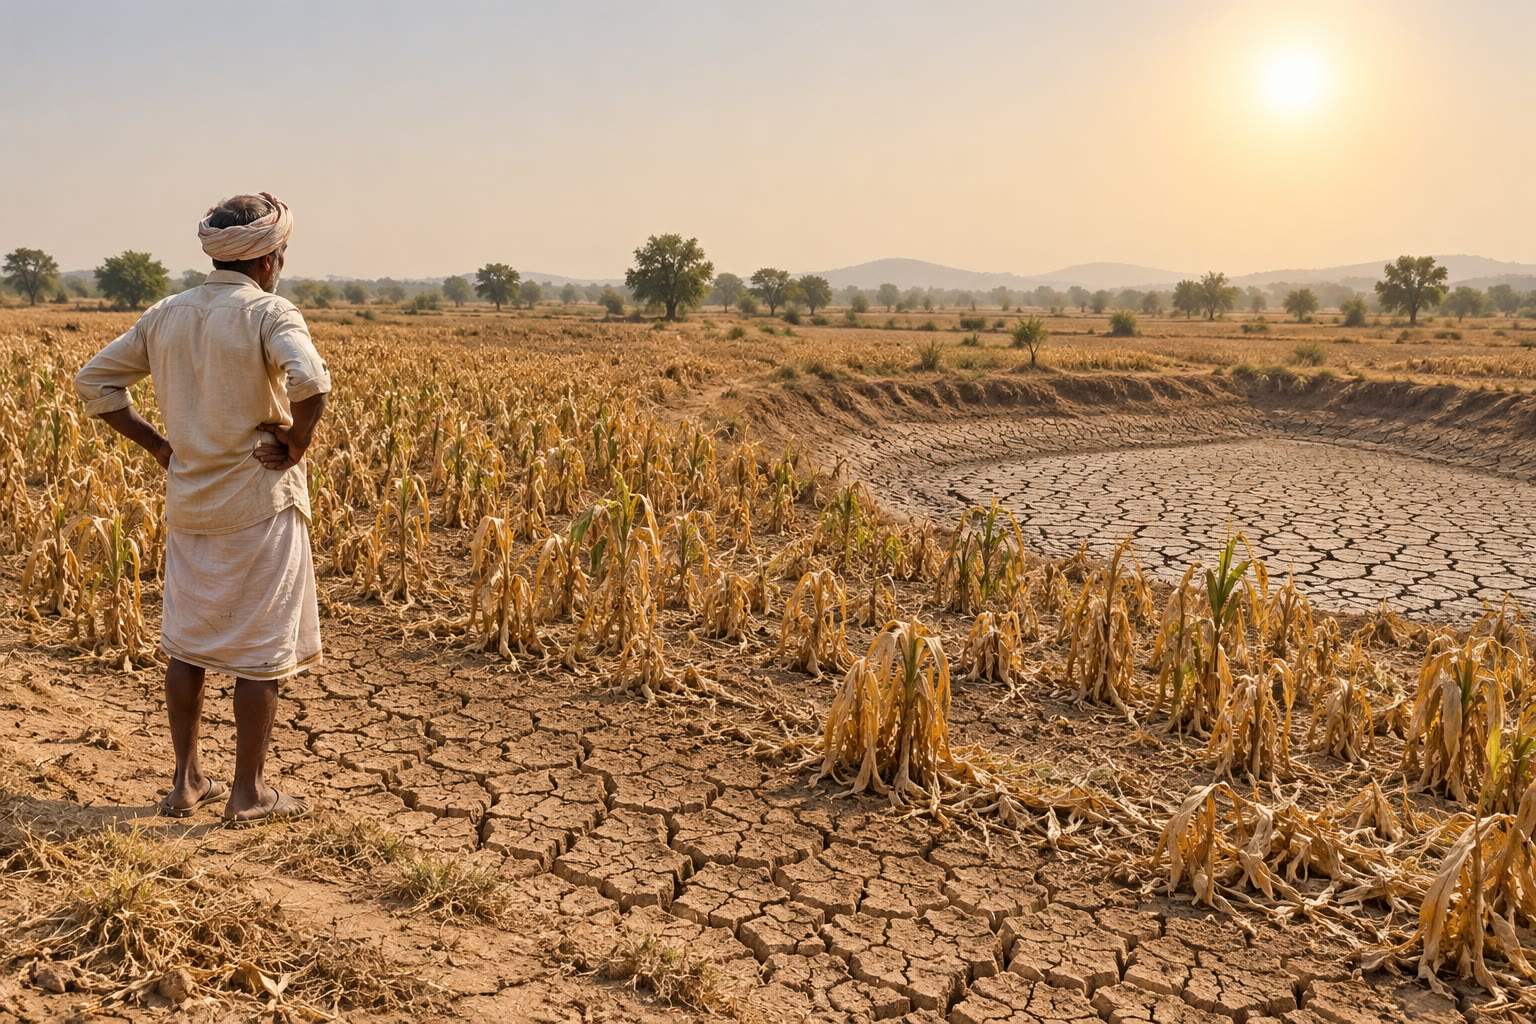
\includegraphics[width=0.42\linewidth]{images/book1/ai/g5-drought-field.jpg}

{\small लंबे सूखे में एक खेत: धरती फट गई है, फ़सलें पीली हैं और तालाब
सूख गया है।}
\end{omfigure}

\section{पानी से आने वाले संकट}

तुम \omterm{def:g1:landscapes-around-us:water}{नदियों} की \omterm{def:g5:water-shapes-the-land:flood}{बाढ़} को पहले से जानते हो (\cref{ch:g5:water-shapes-the-land})।
कई दिनों की \omterm{def:g4:clouds-rain-snow:precipitation}{बारिश} के बाद, या जब \omterm{def:g4:clouds-rain-snow:precipitation}{हिम} तेज़ी से पिघलता है, \omterm{def:g1:landscapes-around-us:water}{नदी} अपने किनारों से ऊपर
उठती है और अपने \omterm{def:g5:water-shapes-the-land:flood}{बाढ़} के \omterm{def:g1:landscapes-around-us:landform}{मैदान} को ढक लेती है। कुछ \omterm{def:g5:water-shapes-the-land:flood}{बाढ़ें} बहुत तेज़ी से आती हैं: किसी
खड़ी ढलान वाली \omterm{def:g1:landscapes-around-us:landform}{घाटी} पर एक ज़ोरदार मूसलाधार \omterm{def:g4:clouds-rain-snow:precipitation}{बारिश} एक घंटे के भीतर एक शांत धारा को
गरजती हुई प्रचंड धारा में बदल सकती है। दूसरी \omterm{def:g5:water-shapes-the-land:flood}{बाढ़ें} \omterm{def:g2:water-on-earth:ocean}{समुद्र} से आती हैं, जब \omterm{def:g5:natural-hazards:storm}{तूफ़ान}
पानी को धकेलकर किसी नीचे \omterm{def:g1:landscapes-around-us:water}{तट} पर चढ़ा देता है।

\section{ज़मीन से आने वाले संकट}

तुम \omterm{def:g4:volcanoes-earthquakes-first-look:earthquake}{भूकंपों} और \omterm{def:g4:volcanoes-earthquakes-first-look:volcano}{ज्वालामुखी} \omterm{def:g4:volcanoes-earthquakes-first-look:eruption}{उद्गारों} को पहले से जानते हो
(\cref{ch:g4:volcanoes-earthquakes-first-look})। ज़मीन से एक तीसरा संकट भी आता है,
और अक्सर पानी उसे छेड़ देता है।

\begin{definition}[भूस्खलन]\label{def:g5:natural-hazards:landslide}
\emph{भूस्खलन}\index{भूस्खलन} \omterm{def:g3:stones-pebbles-sand:rock}{चट्टान}, मिट्टी या \omterm{def:g3:stones-pebbles-sand:sand}{कीचड़} का एक ढेर है जो अचानक किसी
ढलान से नीचे फिसलता या गिरता है।
\end{definition}

लंबी \omterm{def:g4:clouds-rain-snow:precipitation}{बारिशों} से भीगी एक खड़ी ढलान भारी और फिसलन भरी हो जाती है, और वह एक ही बार
में छूट सकती है। \omterm{def:g4:volcanoes-earthquakes-first-look:earthquake}{भूकंप} भी किसी ढलान को हिलाकर ढीला कर सकता है। \omterm{def:g5:natural-hazards:landslide}{भूस्खलन} किसी सड़क
को दबा सकता है, किसी \omterm{def:g1:landscapes-around-us:water}{नदी} को रोक सकता है, या घरों को बहा ले जा सकता है।

\begin{omfigure}
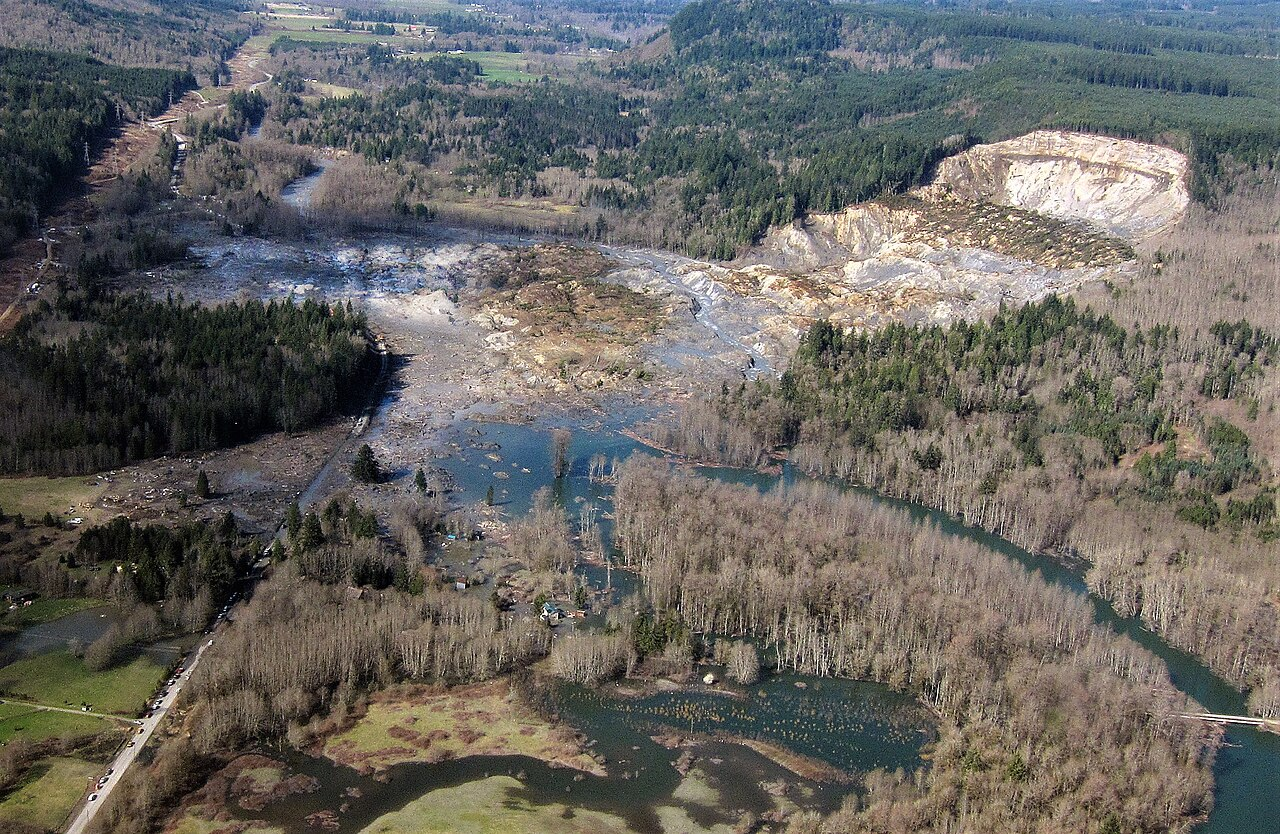
\includegraphics[width=0.6\linewidth]{images/book1/g5-landslide-washington.jpg}

{\small संयुक्त राज्य अमेरिका के वॉशिंगटन राज्य में 2014 का एक बड़ा \omterm{def:g5:natural-hazards:landslide}{भूस्खलन}, एक
विमान से दिखता हुआ। दाईं ओर की \omterm{def:g1:landscapes-around-us:landform}{पहाड़ी} की ढलान ढह गई है; उसका \omterm{def:g3:stones-pebbles-sand:sand}{कीचड़} पूरी \omterm{def:g1:landscapes-around-us:landform}{घाटी} में
फैल गया है, एक सड़क को ढक दिया है और \omterm{def:g1:landscapes-around-us:water}{नदी} को रोक दिया है, जिसने ऊपर की ओर के जंगल में
\omterm{def:g5:water-shapes-the-land:flood}{बाढ़} ला दी है। चित्र: मार्क रीड, अमेरिकी
भूवैज्ञानिक सर्वेक्षण (सार्वजनिक डोमेन)।}\label{fig:g5:natural-hazards:landslide}
% ledger: usgs:oso-aerial
\end{omfigure}

\section{संकट से आपदा तक}

खुले \omterm{def:g2:water-on-earth:ocean}{महासागर} पर एक \omterm{def:g5:natural-hazards:storm}{तूफ़ान}, एक ख़ाली \omterm{def:g5:weather-and-climate:desert}{मरुस्थल} में एक \omterm{def:g4:volcanoes-earthquakes-first-look:earthquake}{भूकंप}, एक ऐसी \omterm{def:g1:landscapes-around-us:landform}{घाटी} में \omterm{def:g5:water-shapes-the-land:flood}{बाढ़} जहाँ
कोई नहीं रहता: ये \omterm{def:g5:natural-hazards:hazard}{प्राकृतिक संकट} हैं, पर ये किसी को नुक़सान नहीं पहुँचाते। यही
घटनाएँ तब ख़तरनाक बनती हैं जब वे वहाँ आती हैं जहाँ लोग रहते हैं।

\begin{definition}[प्राकृतिक आपदा]\label{def:g5:natural-hazards:disaster}
\emph{प्राकृतिक आपदा}\index{प्राकृतिक आपदा} तब होती है जब कोई \omterm{def:g5:natural-hazards:hazard}{प्राकृतिक संकट} ऐसी
जगह पर आता है जहाँ लोग रहते हैं और भारी नुक़सान करता है: लोग घायल होते हैं या मारे
जाते हैं, घर नष्ट होते हैं, सड़कें, पानी और बिजली कट जाती हैं।
\end{definition}

\begin{omfigure}
\begin{tikzpicture}[x=1cm, y=1cm, font=\scriptsize]
  \foreach \dx/\title in {0/{ख़ाली घाटी में बाढ़:\\एक प्राकृतिक संकट},
                          7.6/{वही बाढ़ एक गाँव में:\\एक प्राकृतिक आपदा}} {
    \begin{scope}[xshift=\dx cm]
      % valley sides
      \fill[green!25!brown!30] (0,0) -- (0,2.6) -- (0.4,2.6) -- (1.2,1.0) -- (5.6,1.0)
        -- (6.4,2.6) -- (6.8,2.6) -- (6.8,0) -- cycle;
      \draw[gray!60!black] (0,2.6) -- (0.4,2.6) -- (1.2,1.0) -- (5.6,1.0) -- (6.4,2.6) -- (6.8,2.6);
      % flood water over the whole valley floor
      \fill[blue!30, opacity=0.8] (1.05,1.2) -- (5.75,1.2) -- (5.6,1.0) -- (1.2,1.0) -- cycle;
      \fill[blue!30, opacity=0.8] (1.05,1.2) rectangle (5.75,1.5);
      \draw[blue!60!black] (0.95,1.5) -- (5.85,1.5);
      \node[align=center, anchor=north] at (3.4,-0.1) {\title};
    \end{scope}
  }
  % trees in the empty valley
  \foreach \x in {1.7,2.6,4.4,5.1} {
    \draw[brown!60!black, line width=1pt] (\x,1.0) -- (\x,1.75);
    \fill[green!50!black] (\x,1.95) circle (0.25);
  }
  % houses in the village valley
  \begin{scope}[xshift=7.6cm]
    \foreach \x in {1.6,2.5,3.4,4.3,5.1} {
      \fill[white, draw=black] (\x-0.3,1.0) rectangle (\x+0.3,1.65);
      \fill[red!60!black] (\x-0.38,1.65) -- (\x,2.0) -- (\x+0.38,1.65) -- cycle;
      \fill[blue!30, opacity=0.8] (\x-0.3,1.0) rectangle (\x+0.3,1.5);
    }
    % one house on the high ground, dry
    \fill[white, draw=black] (6.45,2.6) rectangle (6.77,2.95);
    \fill[red!60!black] (6.40,2.95) -- (6.61,3.2) -- (6.82,2.95) -- cycle;
  \end{scope}
\end{tikzpicture}

{\small एक ही \omterm{def:g5:water-shapes-the-land:flood}{बाढ़} दो बार। ख़ाली \omterm{def:g1:landscapes-around-us:landform}{घाटी} में वह किसी को नुक़सान नहीं पहुँचाती; जहाँ
\omterm{def:g5:water-shapes-the-land:flood}{बाढ़} के \omterm{def:g1:landscapes-around-us:landform}{मैदान} पर एक गाँव बसाया गया है, वहाँ वह घरों में पानी भर देती है। ऊँची ज़मीन
पर का घर सूखा रहता है।}
\end{omfigure}

हम \omterm{def:g5:natural-hazards:storm}{तूफ़ान} या \omterm{def:g4:volcanoes-earthquakes-first-look:earthquake}{भूकंप} को रोक नहीं सकते। पर किसी संकट को आपदा बनने से रोकने के लिए हम
बहुत कुछ कर सकते हैं: \omterm{def:g5:water-shapes-the-land:flood}{बाढ़} के \omterm{def:g1:landscapes-around-us:landform}{मैदानों} से और अस्थिर ढलानों के तल से दूर बनाना,
इमारतों को मज़बूत बनाना, \omterm{def:g1:watching-the-weather:weather}{मौसम} और ज़मीन पर नज़र रखना, लोगों को समय पर चेताना, और
सबको सिखाना कि क्या करना है।

\subsection*{चेतावनियाँ}

\omterm{def:g1:watching-the-weather:weather}{मौसम} सेवाएँ दिन-रात आसमान पर नज़र रखती हैं। जब कोई \omterm{def:g5:natural-hazards:storm}{तूफ़ान}, लू या \omterm{def:g5:water-shapes-the-land:flood}{बाढ़} आने वाली
होती है, तो वे रेडियो, टेलीविज़न, फ़ोन और इंटरनेट से चेतावनियाँ भेजती हैं। बहुत-से
देश सबसे शांत से सबसे गंभीर तक रंगों का प्रयोग
करते हैं।

\begin{omfigure}
\begin{tikzpicture}[font=\small, wstep/.style={draw=black!60, minimum width=2.6cm,
    minimum height=0.8cm, font=\small\bfseries, rounded corners=2pt}]
  \node[wstep, fill=green!45] (g) at (0,0) {हरा};
  \node[wstep, fill=yellow!60] (y) at (0.6,0.95) {पीला};
  \node[wstep, fill=orange!70] (o) at (1.2,1.9) {नारंगी};
  \node[wstep, fill=red!65, text=white] (r) at (1.8,2.85) {लाल};
  \node[anchor=west] at ($(g.east)+(0.3,0)$) {कोई ख़ास ख़तरा नहीं};
  \node[anchor=west] at ($(y.east)+(0.3,0)$) {सावधान रहो, ख़बर रखो};
  \node[anchor=west] at ($(o.east)+(0.3,0)$) {तैयार रहो: ख़तरे की संभावना है};
  \node[anchor=west] at ($(r.east)+(0.3,0)$) {बड़ा ख़तरा: अभी क़दम उठाओ, निर्देश मानो};
\end{tikzpicture}

{\small चेतावनी के रंगों की एक सीढ़ी। उनके ठीक-ठीक अर्थ एक देश से दूसरे देश में
अलग होते हैं: चेतावनी के साथ दिए गए निर्देश हमेशा
सुनो।}
\end{omfigure}

\begin{safety}
\textbf{\omterm{def:g5:natural-hazards:storm}{तूफ़ान} में।} घर के अंदर रहो, खिड़कियों से दूर। देखने के लिए बाहर मत जाओ,
और पेड़ों से दूर रहो, जो गिर सकते हैं, और गिरे हुए बिजली के
तारों से भी।

\textbf{\omterm{def:g5:water-shapes-the-land:flood}{बाढ़} में।} ऊँची ज़मीन पर या ऊपर की मंज़िल पर चले जाओ। \omterm{def:g5:water-shapes-the-land:flood}{बाढ़} के पानी में से
कभी पैदल, साइकिल पर या कार में मत जाओ: थोड़ा-सा तेज़ पानी भी तुम्हें गिराने या
किसी कार को बहा ले जाने के लिए काफ़ी है।

\textbf{लू में।} बार-बार पानी पियो, सबसे गरम घंटों में छाँव में या किसी ठंडे कमरे
में रहो, और बूढ़े पड़ोसियों की ख़बर लो।

\textbf{\omterm{def:g4:volcanoes-earthquakes-first-look:earthquake}{भूकंप} में।} झुको, ढको, पकड़े रहो
(\cref{ch:g4:volcanoes-earthquakes-first-look})।

\textbf{हमेशा।} चेतावनियाँ सुनो और ज़िम्मेदार लोग जो कहें, वह तुरंत
करो।
\end{safety}

\section{अभ्यास}

\begin{exercise}[$\star$]\label{exo:g5:natural-hazards:1}
केवल \omterm{def:g5:natural-hazards:hazard}{प्राकृतिक संकट}, या \omterm{def:g5:natural-hazards:disaster}{प्राकृतिक आपदा}?
\begin{enumerate}
  \item[(क)] एक \omterm{def:g4:volcanoes-earthquakes-first-look:earthquake}{भूकंप} एक ख़ाली \omterm{def:g5:weather-and-climate:desert}{मरुस्थल} को हिलाता है।
  \item[(ख)] एक \omterm{def:g5:natural-hazards:storm}{तूफ़ान} किसी शहर के बहुत-से घरों की छतें उखाड़ देता है।
  \item[(ग)] एक \omterm{def:g5:natural-hazards:landslide}{भूस्खलन} पहाड़ों की ऐसी \omterm{def:g1:landscapes-around-us:landform}{घाटी} में गिरता है जहाँ कोई नहीं रहता।
  \item[(घ)] एक \omterm{def:g1:landscapes-around-us:water}{नदी} एक गाँव में \omterm{def:g5:water-shapes-the-land:flood}{बाढ़} ले आती है और उसके घरों में पानी भर देती है।
\end{enumerate}
\end{exercise}

\begin{exercise}[$\star$]\label{exo:g5:natural-hazards:2}
इन संकटों को तीन परिवारों में बाँटो (हवा से, पानी से, ज़मीन से): एक \omterm{def:g5:natural-hazards:landslide}{भूस्खलन};
लू; एक \omterm{def:g5:water-shapes-the-land:flood}{बाढ़}; एक \omterm{def:g4:volcanoes-earthquakes-first-look:volcano}{ज्वालामुखी} \omterm{def:g4:volcanoes-earthquakes-first-look:eruption}{उद्गार}; एक \omterm{def:g5:natural-hazards:storm}{तूफ़ान};
एक \omterm{def:g5:natural-hazards:drought}{सूखा}; एक \omterm{def:g4:volcanoes-earthquakes-first-look:earthquake}{भूकंप}।
\end{exercise}

\begin{exercise}[$\star$]\label{exo:g5:natural-hazards:3}
\omterm{def:g5:natural-hazards:drought}{सूखा} क्या है? दो तरीक़े बताओ जिनसे लंबा \omterm{def:g5:natural-hazards:drought}{सूखा} लोगों को नुक़सान पहुँचाता है।
\end{exercise}

\begin{exercise}[$\star$]\label{exo:g5:natural-hazards:4}
रेडियो आज रात के लिए \omterm{def:g5:natural-hazards:storm}{तूफ़ान} की लाल चेतावनी घोषित करता है। तीन काम बताओ जो तुम्हारे
परिवार को करने चाहिए।
\end{exercise}

\begin{exercise}[$\star$]\label{exo:g5:natural-hazards:5}
आँख वाला एक विशाल घूमता \omterm{def:g5:natural-hazards:storm}{तूफ़ान} एक गरम उष्णकटिबंधीय \omterm{def:g2:water-on-earth:ocean}{समुद्र} के ऊपर बनता है। उसे क्या
कहा जाता है अगर वह (क) उत्तरी अटलांटिक में फ़्लोरिडा के \omterm{def:g1:landscapes-around-us:water}{तट} से टकराए;
(ख) उत्तर-पश्चिमी प्रशांत में जापान से; (ग) हिंद \omterm{def:g2:water-on-earth:ocean}{महासागर} पर भारत के
\omterm{def:g1:landscapes-around-us:water}{तट} से?
\end{exercise}

\begin{exercise}[$\star$]\label{exo:g5:natural-hazards:6}
चेतावनी के चारों रंगों को सबसे शांत से सबसे गंभीर के क्रम में लगाओ। सबसे गंभीर
स्तर पर तुम्हें क्या करना चाहिए?
\end{exercise}

\begin{exercise}[$\star\star$]\label{exo:g5:natural-hazards:7}
पृष्ठ~\pageref{fig:g5:natural-hazards:landslide} पर \omterm{def:g5:natural-hazards:landslide}{भूस्खलन} का फ़ोटो
देखो। बताओ कि \omterm{def:g5:natural-hazards:landslide}{भूस्खलन} ने \omterm{def:g1:landscapes-around-us:landform}{घाटी} के साथ क्या किया: \omterm{def:g1:landscapes-around-us:landform}{पहाड़ी} की ढलान के साथ, सड़क के
साथ और \omterm{def:g1:landscapes-around-us:water}{नदी} के साथ। ऊपर की ओर की ज़मीन अब पानी के नीचे क्यों है?
\end{exercise}

\begin{exercise}[$\star\star$]\label{exo:g5:natural-hazards:8}
टॉम कहता है: ``\omterm{def:g5:water-shapes-the-land:flood}{बाढ़} प्राकृतिक है, इसलिए उसके बारे में कुछ नहीं किया जा सकता।'' लीना
कहती है: ``हम \omterm{def:g1:landscapes-around-us:water}{नदी} को \omterm{def:g5:water-shapes-the-land:flood}{बाढ़} लाने से नहीं रोक सकते, पर \omterm{def:g5:water-shapes-the-land:flood}{बाढ़} को आपदा बनने से रोक सकते
हैं।'' कौन सही है? दो उदाहरणों से समझाओ।
\end{exercise}

\begin{exercise}[$\star\star$]\label{exo:g5:natural-hazards:9}
एक काल्पनिक खेती वाले इलाक़े में आमतौर पर हर महीने लगभग 60 मिलीमीटर \omterm{def:g4:clouds-rain-snow:precipitation}{बारिश} गिरती
है। एक सूखे के दौरान चार महीनों में से हर एक में सामान्य \omterm{def:g4:clouds-rain-snow:precipitation}{बारिश} का केवल एक-चौथाई
गिरा।
\begin{enumerate}
  \item[(क)] चार महीनों में आमतौर पर कितनी \omterm{def:g4:clouds-rain-snow:precipitation}{बारिश} गिरती है?
  \item[(ख)] सूखे के दौरान चार महीनों में कितनी गिरी?
  \item[(ग)] कितनी \omterm{def:g4:clouds-rain-snow:precipitation}{बारिश} कम पड़ी?
\end{enumerate}
\end{exercise}

\begin{exercise}[$\star\star$]\label{exo:g5:natural-hazards:10}
एक काल्पनिक शहर में 1\,200 घर हैं। उनमें से एक-चौथाई उसकी \omterm{def:g1:landscapes-around-us:water}{नदी} के \omterm{def:g5:water-shapes-the-land:flood}{बाढ़} के \omterm{def:g1:landscapes-around-us:landform}{मैदान} पर
बने हैं।
\begin{enumerate}
  \item[(क)] \omterm{def:g5:water-shapes-the-land:flood}{बाढ़} के \omterm{def:g1:landscapes-around-us:landform}{मैदान} पर कितने घर बने हैं?
  \item[(ख)] शहर उनमें से एक-तिहाई घरों के मालिकों को ऊँची ज़मीन पर जाने में मदद
        करता है। \omterm{def:g5:water-shapes-the-land:flood}{बाढ़} के \omterm{def:g1:landscapes-around-us:landform}{मैदान} पर अब भी कितने घर हैं?
\end{enumerate}
\end{exercise}

\begin{exercise}[$\star\star\star$]\label{exo:g5:natural-hazards:11}
दो गाँव, एक-दूसरे से बहुत दूर, एक ही रात में एक ही ताक़त के \omterm{def:g5:natural-hazards:storm}{तूफ़ानों} की चपेट में
आते हैं। पहले में कोई घायल नहीं होता और नुक़सान थोड़ा होता है। दूसरे में बहुत-से
घर नष्ट हो जाते हैं। कम से कम तीन अलग-अलग कारण बताओ जो इस अंतर को समझा
सकें।
\end{exercise}
